\documentclass[13pt]{beamer}

\usepackage[utf8x]{inputenc}
\usepackage[french]{babel}
\usetheme{CambridgeUS}
\usepackage{tikz}
\usepackage[T1]{fontenc} % encodage de la police
\usepackage{graphicx} % affichage des images
\usepackage{animate} % animation d'images
\usepackage[hypcap=false]{caption}
\usepackage{subcaption}
\usepackage{setspace}
\usepackage{tabto}


\title[Présentation]{\textbf{Conception Logiciel}}
\subtitle[\ldots]{Projet SOKOBAN}
\author[Eloi, Erwann, Emile]{
	\textbf{LEDOUX Eloi},\\
	\textbf{TAUPIN Erwann},\\
	\textbf{KITSOUKOU Manne Emile},\\
	\emph{L1 informatique, Groupe 2B},\\}
\institute[Unicaen]{Université Caen-Normandie}



\begin{document}

\frame{\titlepage}

\begin{frame} % Table des matières
    \frametitle{Table des matières}
    \tableofcontents
\end{frame}

\section{Travaux préléminaires}
\begin{frame}
    \frametitle{Travaux préliminaires}
    Ils se sont articulés autour de trois(3) points:
    \begin{itemize}
        \item Les renseignements sur le projet - Qu'est-ce qu'un Sokoban?
        \item La répartition des fichiers
        \item La répartition des tâches au sein du groupe
    \end{itemize}
\end{frame}

\section{Structure du projet}

\begin{frame}
    Les étapes pour aboutir à une version fonctionnelle en console:
    \begin{itemize}
        \item Création d'un fichier grille
        \item Lecture d'un niveau de sokoban (fichier .sok)
        \item Adaptation des symboles du programme
    \end{itemize}
\end{frame}
\begin{frame}
    \frametitle{Version jouable en Console}
    Implémentations des déplacements:
    \begin{itemize}
        \item Déplacements du personnages
        \item Déplacements des caisses
        \item Conditions de victoire
    \end{itemize}
\end{frame}

\section{Aspect graphique}
\subsection{Approche}
\begin{frame}
    \frametitle{Aspect graphique}
    Pour gérer l'aspect graphique nous nous appuyons sur une programmation événementielle à l'aide du module Pygame.
    \begin{figure}
        
\includegraphics[scale=0.2]{images/Pygame_(2019)_Logo.png}
    \end{figure}
\end{frame}

\subsection*{Les événements}
\begin{frame}
    \frametitle{Aspect graphique}
    Les événements utilisateurs:
    \begin{itemize}
        \item \textbf{JOUER}
        \item \textbf{GO\_MENU}
        \item \textbf{RUN\_SOLUTION}
        \item \textbf{ECRAN\_FIN}
        \item \textbf{NIVEAUX}
        \item \textbf{AUTOMATIQUE}
    \end{itemize}
\end{frame}

\subsection{Les couches}
\begin{frame}
    \frametitle{Les couches}
    Qu'appelons nous par couche ? \\
    \medskip
    Une couche est un objet possédant des données,
    des informations pouvant être manipulées et modifiées à travers deux(2) méthodes:
    \begin{itemize}
        \item \textbf{react\_to}
        \item \textbf{draw}
    \end{itemize}
	\medskip
    Les couches intermédiaires:
    \begin{itemize}
        \item Le menu
        \item La sélection des niveaux
        \item La couche de fin
    \end{itemize}

\end{frame}

\begin{frame}
    \frametitle{La couche JEU}
    La couche JEU permet de gérer la partie de jeu.
    \begin{figure}
        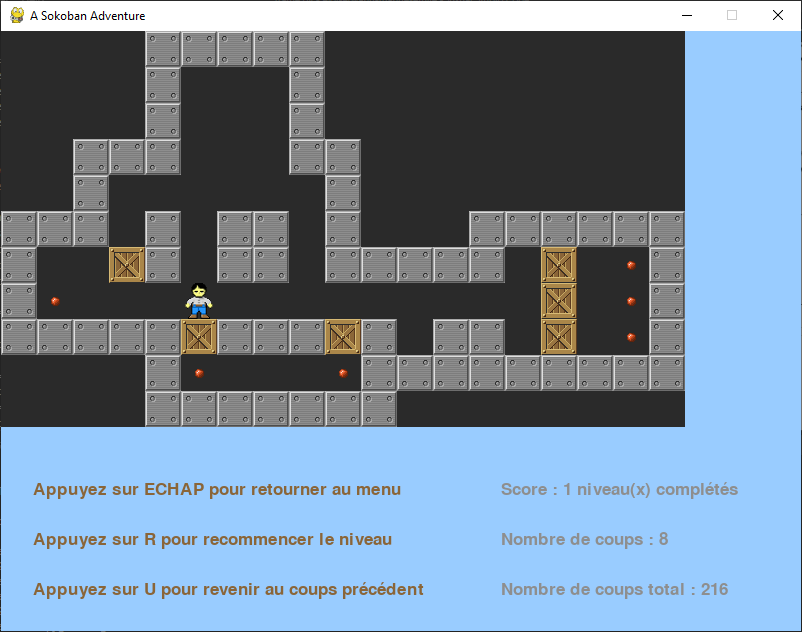
\includegraphics[scale=0.4]{images/Capture_104539.png}
    \end{figure}
\end{frame}

\begin{frame}
    \frametitle{La couche JEU}
    Pour afficher le plateau de jeu d'un niveau de SOKOBAN, il est nécessaire d'utiliser l'objet \textbf{Image}.
    \\
    L'objet \textbf{Image} permet, à partir d'un tableau 2D (liste de liste ou niveau SOKOBAN), de dessiner ces éléments.\\
    Cela s'effectue grâce à la méthode \textbf{dessine\_grille} ou \textbf{dessine\_level}.
\end{frame}

\begin{frame}
    \frametitle{Fonctionnement des méthodes d'affichage d'un tableau 2D}
    \textbf{\emph{Début de la méthode:
                    \\
                    \bigskip 
                    \tabto{2em}itération sur les éléments du tableau 2D (par ligne et colonne ou par numéro de case):
                    \\
                    \tabto{3em} tester si le caractère est dans le dictionnaire des caractères prédéfinis
                    \\
                    \tabto{4em} afficher le caractère sur l'écran à des coordonnées calculées selon sa position dans le tableau
                    \\
                    \bigskip 
                    Fin de la méthode}}
\end{frame}
\section{L'algorithme de recherche}
\begin{frame}
    \frametitle{Recherche d'un solveur compatible}
    Comme nous n'avions plus beaucoup de temps à consacrer à la création d'un solveur, nous avons fait le choix de procéder, non pas à l'écriture d'un algorithme mais, à l'intégration d'un algorithme déjà existant.
    
    \medskip
    
    Le solveur choisi a été écrit par \textit{KnightofLuna} (\href{https://github.com/KnightofLuna/sokoban-solver}{lien GitHub du projet}).
    
    \medskip
    
    Ce solveur peut utiliser quatre(4) algorithmes différents : A*, BFS, DFS, UCS.
    
    \medskip
    
    Cependant, pour notre projet, nous avons choisi de ne conserver que l'algorithme A*.
\end{frame}

\begin{frame}
	\frametitle{L'algorithme de recherche}
	Comment fonctionne un algorithme de recherche ?
	
	\medskip
	
	L'algorithme A* est un algorithme de recherche de chemin dans un graphe, de plus c' est un algorithme itératif.
	
	\medskip
	
	Le A* donne rapidement une assez bonne solution, cependant cette solution n'est pas toujours optimale (cf. annexe C du rapport).
	
	\medskip
	
	À chaque coup, il va essayer de se rapprocher de la destination par le chemin le plus direct possible.
	
	\begin{center}
		\animategraphics[width=90px, autoplay, loop]{12}{images/AstarAnimation/AstarAnimation-}{0}{200}
		
		{\tiny $\copyright$ Subh83 sur Wikipédia}
		
	\end{center}
\end{frame}

\begin{frame}
    \frametitle{Intégration de l'algorithme}
    Modifications apportées :
    \begin{itemize}
        \item Remplacement des caractères utilisés par l'algorithme 
        \item Ajout de la possibilité pour le personnage d'être sur un objectif
        \item Remplacement des lettres qui définissent les actions possibles
    \end{itemize}
\end{frame}

\begin{frame}
    \frametitle{Intégration de l'algorithme}
    Comment l'algorithme fonctionne dans le programme ?\\
    La résolution s'effectue par changement de couche.
    Cette couche fonctionne selon ces points:
    \begin{itemize}
        \item Recherche des solutions lors de l'initialisation
        \item Lance la résolution dans la méthode \textbf{react\_to}
        \item Affiche le plateau grâce à la méthode \textbf{draw}
    \end{itemize}
\end{frame}

\section{Les fonctionnalités ajoutées}
\begin{frame}
    \frametitle{Les fonctionnalités ajoutées}
    Les divers ajouts que nous avons pu implémenter :
    \begin{itemize}
        \item Le son
        \item Les ajouts textuelles
        \item Les fonctionnalités de "sauvetages" dans une partie:
        \begin{itemize}
            \item Le Undo: retour en arrière
            \item Le Reset: Réinitialiser la partie en cours
        \end{itemize}
    \end{itemize}
\end{frame}

\section{Conclusion}
\begin{frame}
    \frametitle{Conclusion}
    Un travail formateur, tant pour la programmation que le travail en équipe.
    \\
    \bigskip
    Un travail qui reste néanmoins améliorable sur de nombreux points :
    \begin{itemize}
        \item Avec l'ajout d'un intégrateur de niveaux directement en jeux.
        \item Avec une possibilité de résolution par l'algorithme plus poussée et simultanée.
        \item Avec la possibilité de jouer à plusieurs en comparant ses meilleurs scores sauvegardés par le jeu.
    \end{itemize}
\end{frame}

\end{document}